\aufgabe 2


Counterexample: 

\begin{figure}[h]
	\centering
	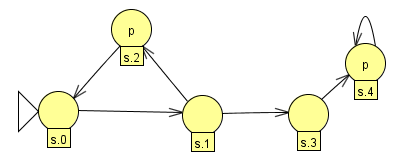
\includegraphics[width=0.7\textwidth]{Gegenbeispiel.png}
\end{figure}

While the CTL formulae $AXAFp$ is accepted by the example above. The path $s_0s_1s_3$ however is not accepted by the formular $AFAXp$. Thus $AXAFp$ and $AFAXp$ are not equivalent.

%\begin{align*}
%	& \mathcal{L},\sigma\vDash\mathcal{AXAF}p \\
%	\Leftrightarrow & \forall\pi=\sigma s_1...: \pi\vDash\mathcal{XAF}p \\
%	\Leftrightarrow & \forall\pi=\sigma s_1...: s_1\vDash\mathcal{AF}p \\
%	\Leftrightarrow & \forall\pi=\sigma s_1...: \forall\tilde{\pi}=s_1s_2...:\mathcal{F}p \\
%	\Leftrightarrow & \forall\pi=\sigma s_1...: \forall\tilde{\pi}=s_1s_2...:\exists j\ge 0:s_j\vDash p \\
%	\Leftrightarrow & \forall\pi=\sigma s_1...: \exists j\ge 0:\forall \tilde{\pi}=s_js_{j+1}...: s_{j+1}\vDash p \\
%	\Leftrightarrow & \forall\pi=\sigma s_1...: \exists j\ge 0:\forall \tilde{\pi}=s_js_{j+1}...: s_j\vDash \mathcal{X}p \\
%	\Leftrightarrow & \forall\pi=\sigma s_1...: \exists j\ge 0:s_j\vDash \mathcal{AX}p \\
%	\Leftrightarrow & \forall\pi=\sigma s_1...: \pi\vDash \mathcal{FAX}p \\
%	\Leftrightarrow & \mathcal{L},\sigma\vDash\mathcal{AFAX}p \\
%\end{align*}